% !TeX root = report.tex
% !TeX spellcheck = en_GB

\section{Experiment}
The problem definition is as follows: 
Given a graph $G$, a source vertex $s$, and a goal vertex $t$, find the shortest path from $s$ to $t$ in $G$.

\newpar We have restricted the problem to instances where a path between $s$ and $t$ exists.

\subsection{Instances}
In order to feed the instance into the network, we use an encoding of the adjacency matrix of the graph, where each edge has the value 1, and each non-edge has the value 0. The source and goal vertices are one-hot encoded. See \autoref{fig:input:encoding} for an example. The output of the ENTM is interpreted as a one-hot encoding of the next vertex on the path to the goal.

\begin{figure}[ht]
	\centering
	\begin{subfigure}{.5\textwidth}
		\centering
		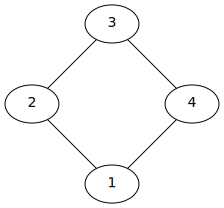
\includegraphics[width=\textwidth]{figures/encoding.png}
		\subcaption{}
	\end{subfigure}%
	\begin{subfigure}{.5\textwidth}
		\centering
		\begin{tabular}{|c|c|c|c|c|}
			\hline
			&\textbf{1}&\textbf{2}&\textbf{3}&\textbf{4}\\\hline
			\textbf{1}&0&1&0&0\\\hline
			\textbf{2}&1&0&1&1\\\hline
			\textbf{3}&0&1&0&1\\\hline
			\textbf{4}&0&1&1&0\\\hline
		\end{tabular}
		\subcaption{}
	\end{subfigure}\par\bigskip
	\begin{adjustbox}{center}
		\begin{subfigure}{1.3\textwidth}
			\centering
			\begin{tabu}{|c|c|c|c||c|c|c|c||c|c|c|c||c|c|c|c|[2pt]c|c|c|c|[2pt]c|c|c|c|}
				\hline
				0&1&0&0&1&0&1&1&0&1&0&1&0&1&1&0&1&0&0&0&0&0&0&1\\\hline
			\end{tabu}
			\subcaption{}
		\end{subfigure}
	\end{adjustbox}
	\caption{(a) Shows a simple graph, (b) its adjacency matrix and (c) an encoding of the entire instance where $s=1$ and $t=4$. The three structures are the flattened adjacency table, the one-hot encoding of $s$, and the one-hot encoding of $t$}
	\label{fig:input:encoding}
\end{figure}

\newpar The instances are generated in a manner which tries to avoid over fitting and support general solutions. This is done by using randomly generated graphs with certain restrictions. The graph must contain a path of a given length to ensure a certain level of complexity. This level of complexity filters out optimal strategies on non general case graphs such as graphs with paths of length 1 where the optimal solution is outputting the goal vertex. Generating these graphs is done by picking two random vertices $ s $ and $ t $ and randomly pick vertices that forms a path from $ s $ to $ t $. The remaining vertices are then connected to the set of explored vertices randomly. This ensures that the ENTM cannot just follow edges but need to explore branches of the graph. The generated graphs are of fixed size to ensure neural network compatibility.

\subsection{Fitness}
The fitness function is defined as a summation of scores for the output of each step on the shortest path. A function $ DistTo(u) $ returns the distance from vertex $ u $ to the goal vertex. The vertex $ current $ describes the vertex which was given to the network and $ next $ denotes the networks choice of next vertex. The following scores are given in each step:

\begin{itemize}
	\item[] 1 point: if $ DistTo(next) > DistTo(current) $
	\item[] 2 points: if $ DistTo(next) = DistTo(current) $
	\item[] 4 points: if $ DistTo(next) < DistTo(current) $
\end{itemize}

\noindent In the case that one step resulted in a move where no edge exists the overall score is set to 0. No further steps are performed.

\newpar The motivation these scores is to reward neural networks that understand the underlying graph problem more than a network that chooses arbitrarily.

\newpar The final score is normalized by dividing the score with the maximum score which is $ DistTo(source)*4 $.

\subsection{The Experiments}
To assess and measure how well the shortest path problem is solved, four times three experiments are performed. The first three experiments uses the NEAT framework to train and build neural networks with recurrent connections. The next three experiments uses the ENTM extension of the NEAT framework and can therefore in addition approximate Neural Turing machines. These experiments are still using recurrent neural networks. The memory is unlimited (within the bounds of the host machine), the write vector size is 4 and the default jump mechanism introduced in \cite{luders2017continual} is used. Then we repeat all experiments, with the only difference that the neural networks are required to be acyclic.

\newpar All experiments uses the exact same configuration for NEAT and the general problem to make it easier to compare them. Each configuration uses 30 species and a population of 500. Each phenotype is tested on 25 unique graphs per generation. An example configuration can be seen in \autoref{appendix:sharpneat:configurations}. The appendix also contains the changes between the different experiments.

%\newpar With these encodings for input and output, we can supply the same graph and goal, multiple times, while only changing the current source vertex. The neural network will then return its answer to the next vertex on the path, that can then be used as a new source vertex.